\chapter{BitBucket Data Center}


\section{Webhook Configuration}

BitBucket Data Center can assign web hooks at the Project (aka Organization) level as well as at the
repository level.  Deploying web hook configurations for an enterprise-scale SCM is generally better
at the organization level since it will apply to all repositories in the organization.  Deploying
at the repository level is mostly suitable for testing purposes only.

Figure \ref{fig:bbdc-project-config} shows the BitBucket Data Center project configuration screen.  The
project key will appear in clone URLs and can be used as part of the regular expression 
placed in the \texttt{repo-match} configuration element.  Please see Section \ref{sec:scm-block-element} 
for a description of the \texttt{repo-match} configuration element.

The project's "Webhooks" configuration can be used to configure the \cxoneflow endpoint that will receive
the webhook events for each repository in the organization.  The \texttt{/bbdc} endpoint should be used
so the \cxoneflow endpoint understands the format of the event payload so it can properly orchestrate the
scan workflow. 

\begin{figure}[h]
    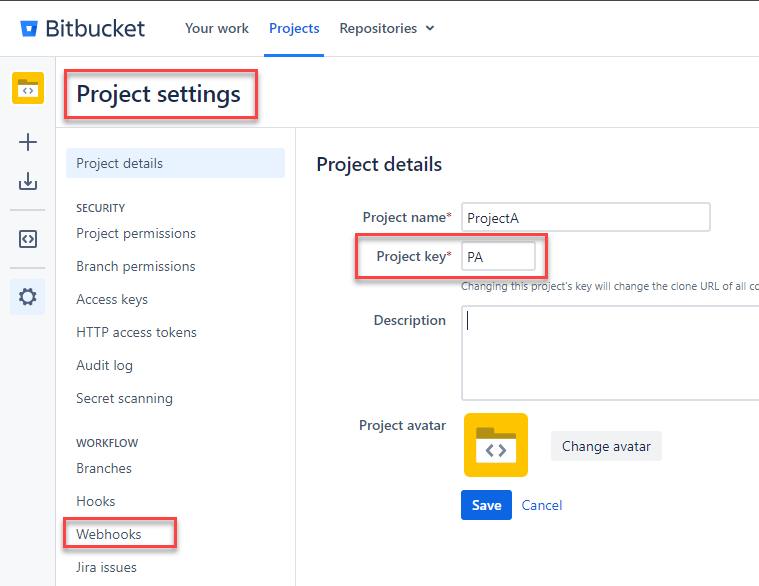
\includegraphics[width=\textwidth]{graphics/bbdc-project-config.png}
    \caption{BitBucket Data Center Project Configuration}
    \label{fig:bbdc-project-config}
\end{figure}

\begin{figure}[h]
    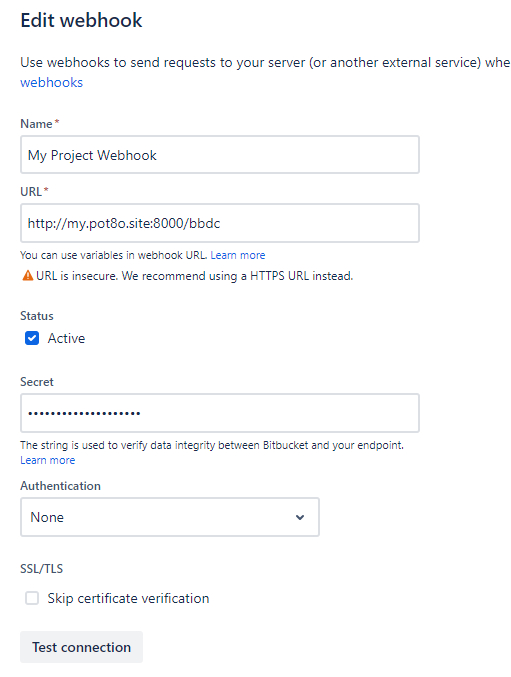
\includegraphics[width=\textwidth]{graphics/bbdc-webhook-config.png}
    \caption{BitBucket Data Center Webhook Configuration}
    \label{fig:bbdc-webhook-config}
\end{figure}



Figure \ref{fig:bbdc-webhook-config} shows a typical webhook configuration.  The Secret is how \cxoneflow
validates the origin of the event payload.  The configuration element \texttt{shared-secret}, as described
in Section \ref{sec:connection-element}, should be configured with the webhook secret value.  If \cxoneflow
is running at the specified URL endpoint, the "Test Connection" button will send a diagnostic ping
and receive back a positive response.  If the connection test fails, please ensure that \cxoneflow is running
at the address specified in the URL field and that the BitBucket Data Center server can make a connection
to that URL.

If the webhook is configured at the Project level, the events sent apply to all repositories contained
within the project.  Figure \ref{fig:bbdc-repo-event-config} shows the configured repository-level webhook 
events that will send a webhook payload to the \cxoneflow endpoint. 
Figure \ref{fig:bbdc-pr-event-config} shows the configured pull-request events that will be sent to 
the \cxoneflow endpoint.  The following events are currently supported:


\pagebreak
\begin{itemize}
    \item Repository Events
        \begin{itemize}
            \item Push
        \end{itemize}
    \item Pull Request Events
        \begin{itemize}
            \item Scanning Orchestration (Required)
                \begin{itemize}
                    \item Opened
                    \item Source branch updated
                    \item Modified
                \end{itemize}
        \end{itemize}
        \begin{itemize}
            \item Pull Request Scan Tagging (Optional)
                \begin{itemize}
                    \item Approved
                    \item Changes requested
                    \item Declined
                    \item Unapproved
                    \item Merged
                    \item Deleted
                \end{itemize}
        \end{itemize}

\end{itemize}


\begin{figure}[h]
    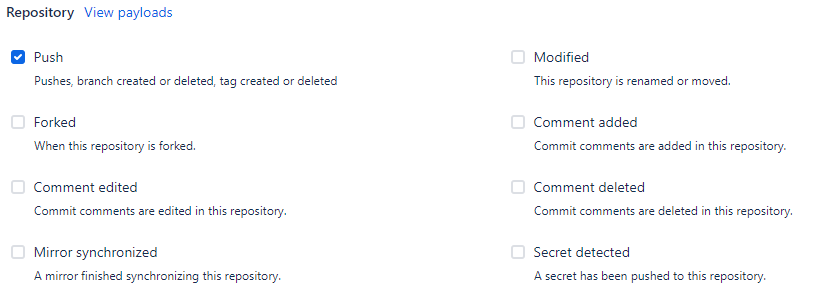
\includegraphics[width=\textwidth]{graphics/bbdc-repository-event-config.png}
    \caption{BitBucket Data Center Webhook Repository Event Config}
    \label{fig:bbdc-repo-event-config}
\end{figure}

\begin{figure}[h]
    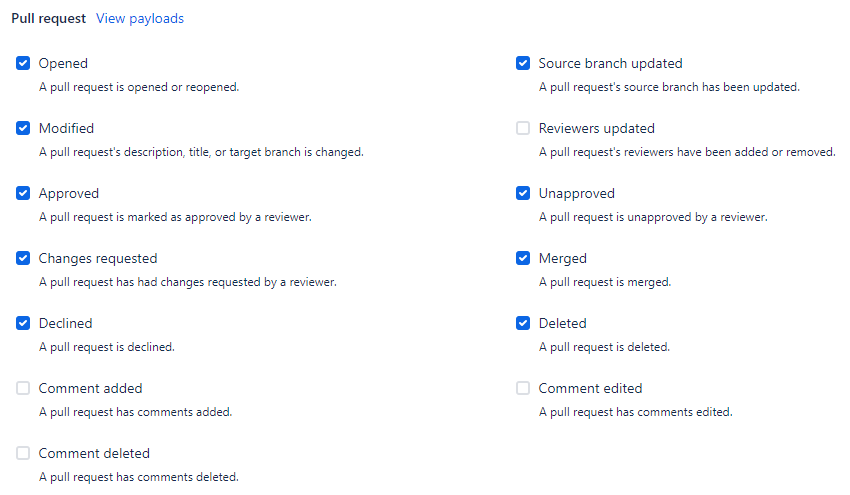
\includegraphics[width=\textwidth]{graphics/bbdc-pr-event-config.png}
    \caption{BitBucket Data Center Webhook Pull Request Event Config}
    \label{fig:bbdc-pr-event-config}
\end{figure}


\section{\cxoneflow HTTP Access Tokens}

While it is possible to use Basic Authorization to access the SCM, typically this is a configuration that
should be avoided.  The Basic Authorization is typically an interactive user account that can be subject
to password changes and Captcha verification that can break \cxoneflow operations.  It is generally
best to use a project-level HTTP Access Token for SCM connection configurations \texttt{api-auth} or
\texttt{clone-auth}.  Please refer to Section \ref{sec:connection-element} for more details about the token
configuration.

Figure \ref{fig:bbdc-token-config} shows the project-level "HTTP Access tokens" configuration.  The required
token permissions for \cxoneflow operations are:

\begin{itemize}
    \item Project read
    \item Repository read\footnote{Figure \ref{fig:bbdc-token-config} shows "Repository write".  There may be future versions of \cxoneflow that will need to create pull-request comments which will require write access.  If desired, the token can be granted "Repository read" until a write capability is released.}
\end{itemize}


\begin{figure}[h]
    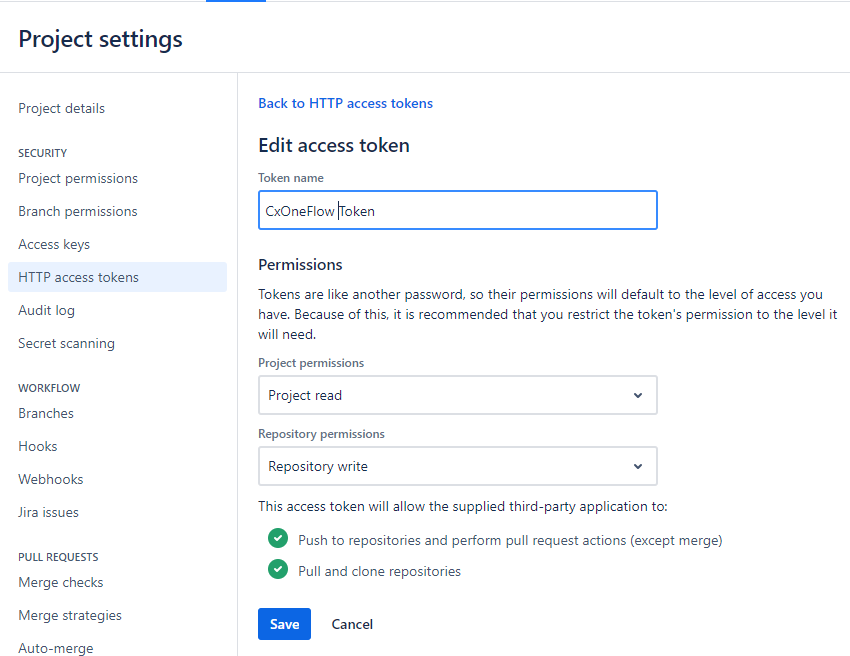
\includegraphics[width=\textwidth]{graphics/bbdc-token-config.png}
    \caption{BitBucket Data Center Project-Level HTTP Access Token Config}
    \label{fig:bbdc-token-config}
\end{figure}


\section{Protected Branches}

The \cxoneflow workflow, as described in Section \ref{sec:overview}, uses the concept of "Protected Branches"
to know when to invoke workflows.  BitBucket Data Center allows for the configuration of the branching model
at the project and repository level.  Some repositories inherit their branching model from the project
configuration, but the ability for this to be overridden at the repository level is an optional configuration.
The branching model is used to determine which branches are "Protected Branches".

The project-level branching model configuration is shown in Figure \ref{fig:bbdc-branch-config}.  The
repository-level branching model configuration is similar in that both allow the definition of
"Development" and "Production" branches.  \cxoneflow considers any branch specified as a Development
or Production branch to be a "Protected Branch".

\begin{figure}[h]
    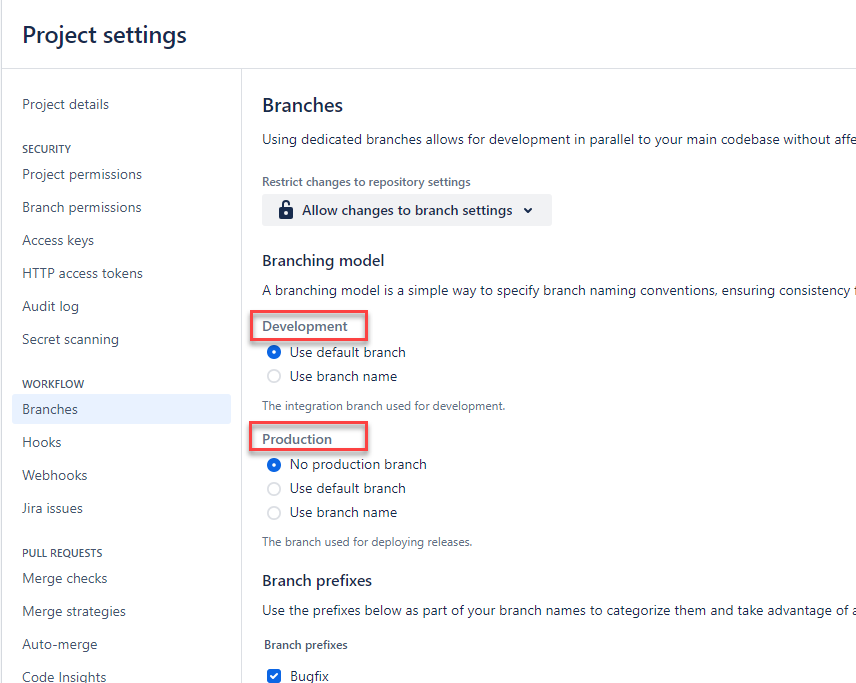
\includegraphics[width=\textwidth]{graphics/bbdc-branch-config.png}
    \caption{BitBucket Data Center Project-Level Branch Config}
    \label{fig:bbdc-branch-config}
\end{figure}

